\documentclass[15pt]{scrartcl}
\usepackage[sexy]{evan}
\newcommand{\R}{\mathbb{R}}
\newcommand{\N}{\mathbb{N}}
\newcommand{\Q}{\mathbb{Q}}
\newcommand{\Z}{\mathbb{Z}}
\newcommand{\F}{\mathbb{F}}
\usepackage{relsize}
\setcounter{secnumdepth}{0}
\usepackage{pgfplots}
\pgfplotsset{compat=1.18, width=10cm}


\begin{document}
\title{Tikz Notes}
\date{\today}
\author{Jiawen Huang}
\maketitle

\tikz \draw[<-] (0,0) -- (1,2) -- (2,0);

\begin{tikzpicture}
    \draw (0,0) circle (1);
    \draw (2,0) circle (1.5in);
    \draw (4,0) ellipse (1 and 5);
    \draw (0,0) rectangle (5,4);
    \draw (0,0) grid (5,4);
    \draw node at (3,0){$V(X^2)$};
    \filldraw (6,2)--(8,7) node[anchor=east] {Filled Circle};
\end{tikzpicture}
\newpage


\begin{center}
    
\begin{tikzpicture}[transform canvas={scale=4.0}]
        \filldraw[red] (0,0) circle (0.05cm);
        \draw[blue] (0,0) arc (90:-90:0.5cm and 1cm);
        \shade[ball color=blue!20!green, opacity=0.1] (0,-2) circle (1cm);
    \end{tikzpicture}
\end{center}
\newpage 

\begin{center}
    \begin{tikzpicture}[Kai/.style={rectangle, draw=red, fill=white!90!red, thick, minimum size=7mm}]
        \node[Kai] (A) {First};
        \node[Kai] (B) [below=of A] {Second};
        \node[Kai] (C) [below=of B]{Third};

        \draw[->, thick] (A.south)  to node[right]{$a$}(B.north);
        \draw[->, thick] (B.south) -- (C.north);
        \draw[->, thick] (C.east) .. controls +(right:7mm) and +(right:30mm) .. (A.east);
    \end{tikzpicture}
\end{center}
\section{Tikz}

\tikz \draw[->] (0,0) -- (2,1) -- (3,2);

\begin{tikzpicture}
\draw (0,0) circle (1);
\draw (2,0) circle (1.5in);
\draw (5,0) ellipse (10pt and 20 pt);

\draw node at (3,0) {$f(x)$};

\filldraw (6,0) circle (0.1cm) node[anchor=west]{Anchored Node};

\end{tikzpicture}

\vspace{1in}

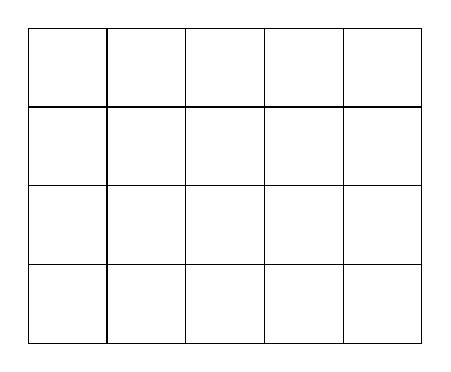
\begin{tikzpicture}
\draw (0,0) rectangle (5,4);
\draw (0,0) grid (5,4);
\end{tikzpicture}

%%Various Line Thickness

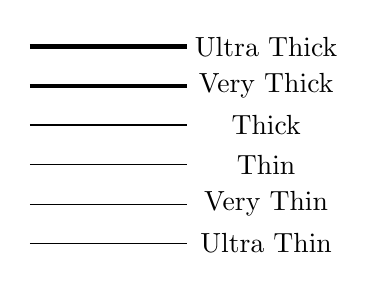
\begin{tikzpicture}
\draw[ultra thick] (0,3) -- (2,3);
\draw[very thick] (0,2.5) -- (2,2.5);
\draw[thick] (0,2) -- (2,2);
\draw[thin] (0,1.5) -- (2,1.5);
\draw[very thin] (0,1) -- (2,1);
\draw[ultra thin] (0,.5) -- (2,.5);

\draw node at (3, 3) {Ultra Thick};
\draw node at (3, 2.5) {Very Thick};
\draw node at (3, 2) {Thick};
\draw node at (3, 1.5) {Thin};
\draw node at (3, 1) {Very Thin };
\draw node at (3, 0.5) {Ultra Thin};
\end{tikzpicture}



\newpage

	\begin{center}
		
\begin{tikzpicture}[transform canvas={scale=4.0}]  %%[scale=4] ONLY changes distances, not the canvas
		\draw[blue] (0,1) arc (90:-90:0.5cm and 1cm);
		\draw[dashed, red] (0,1) arc (90:270:0.5cm and 1cm);
		\draw (0,0) circle (1cm);
		\filldraw[red] (0,1) circle  (0.05); %add fill=, and draw= to have separate colours
		\filldraw[red] (0,-1) circle (0.05);
		\shade[ball color=blue!10!white,opacity=0.20] (0,0) circle (1cm);
		\end{tikzpicture}
	\end{center}

\vspace{2in}


\begin{tikzpicture}[
SIR/.style={rectangle, draw=red!60, fill=red!5, very thick, minimum size=5mm},
]
%Nodes
\node[SIR]    (Susceptible)                              {Susceptible $S(t)$};
\node[SIR]    (Infectious)       [below=of Susceptible] {Infectious $I(t)$};
\node[SIR]    (Recovered)       [below=of Infectious] {Recovered $R(t)$};

%Lines
\draw[->, very thick] (Susceptible.south)  to node[right] {$a$} (Infectious.north);
\draw[->, very thick] (Infectious.south)  to node[right] {$b$} (Recovered.north);
\draw[->, very thick] (Recovered.east) .. controls  +(right:7mm) and +(right:7mm)   .. (Susceptible.east);

\end{tikzpicture}
\vspace{1in}

\begin{tikzpicture}[
youngnode/.style={rectangle, draw=red!60, fill=red!5, very thick, minimum size=40},
oldnode/.style={rectangle, draw=blue!60, fill=blue!5, very thick, minimum size=40},
]
%Nodes
\node[oldnode]        (SusO)                            { $S_O(t)$};
\node[oldnode]        (InfO)       [below=of SusO]      { $I_O(t)$};
\node[oldnode]        (RecO)       [below=of InfO]      { $R_O(t)$};

\node[youngnode]      (SusY)        [left=of SusO]      { $S_Y(t)$};
\node[youngnode]      (InfY)        [left=of InfO]      { $I_Y(t)$};
\node[youngnode]      (RecY)        [left=of RecO]      { $R_Y(t)$};

%Lines
\draw[->, very thick] (SusO.south east)  to node[right] {$a_{OO}$} (InfO.north east);
\draw[->, very thick] (InfO.south)  to node[right] {$b_O$} (RecO.north);
\draw[->, very thick] (RecO.east)  .. controls  +(right:17mm) and +(right:17mm)   .. (SusO.east);

\draw[->, very thick] (SusY.south west)  to node[left] {$a_{YY}$} (InfY.north west);
\draw[->, very thick] (InfY.south)  to node[left] {$b_Y$} (RecY.north);
\draw[->, very thick] (RecY.west) .. controls  +(left:17mm) and +(left:17mm)   .. (SusY.west);

\draw[dashed,->, very thick] (InfO.north west)  to  (SusY.south east);
\draw[->, very thick] (SusY.south east)  to node[left] {$a_{OY}$} (InfY.north east);

\draw[->, very thick] (SusO.south west)  to node[right] {$a_{YO}$} (InfO.north west);
\draw[dashed,->, very thick] (InfY.north east)  to  (SusO.south west);
\end{tikzpicture}


\section{2D}
\begin{tikzpicture}
    \begin{axis}[xmin=-2, xmax=2, ymin=-2, ymax=2, hide axis]
        \addplot[color=red, dashed, mark=*, samples=20]{x^2};
        \addplot[color=blue]{1-x^2};
    \end{axis}
\end{tikzpicture}

\begin{tikzpicture}
    \begin{axis}[hide axis]
        \addplot[]{x^2};
        \addplot[color=blue]{1-x^2};
    \end{axis}
\end{tikzpicture}

\begin{tikzpicture}
    \begin{axis}[axis lines=middle]
        \addplot[domain=-3:3]{x^2};
        \addplot[color=blue]{1-x^2};
    \end{axis}
\end{tikzpicture}

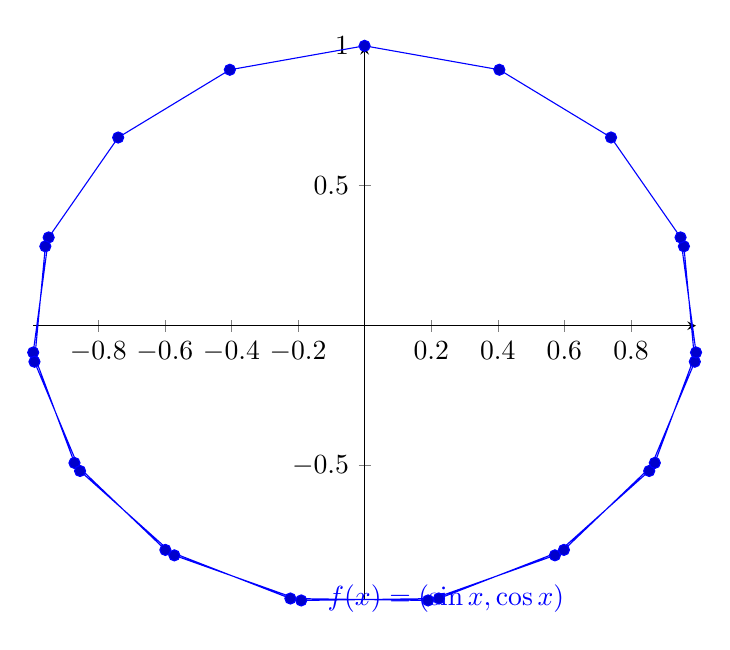
\begin{tikzpicture}
    \begin{axis}[axis lines=middle, clip=false]
        \addplot+[]({sin(deg(x))},{cos(deg(x))}) node[right, pos=0.2]{$f(x)=(\sin x, \cos x)$};
    \end{axis}
\end{tikzpicture}

\newpage
\begin{tikzpicture}
    \begin{axis}[clip=false, xmin=0, xmax=2.5*pi, xtick={0,pi/2,pi,3*pi/2,2*pi}, axis lines=middle, xticklabels={0,$\frac{\pi}{2}$,$\pi$,$\frac{3\pi}{2}$,$2\pi$},]
        \addplot[domain=0:2*pi, red]{sin(deg(x))} node[right, pos=0.9]{$f(x)=\sin x$};
    \end{axis}
\end{tikzpicture}

\section{3D}
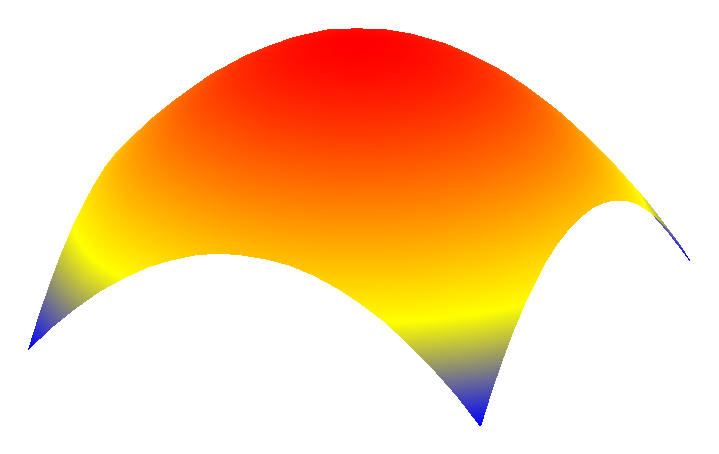
\begin{tikzpicture}
    \begin{axis}[hide axis]
        \addplot3[surf, samples=20, shader=interp]{1-x^2-y^2};

    \end{axis}
\end{tikzpicture}
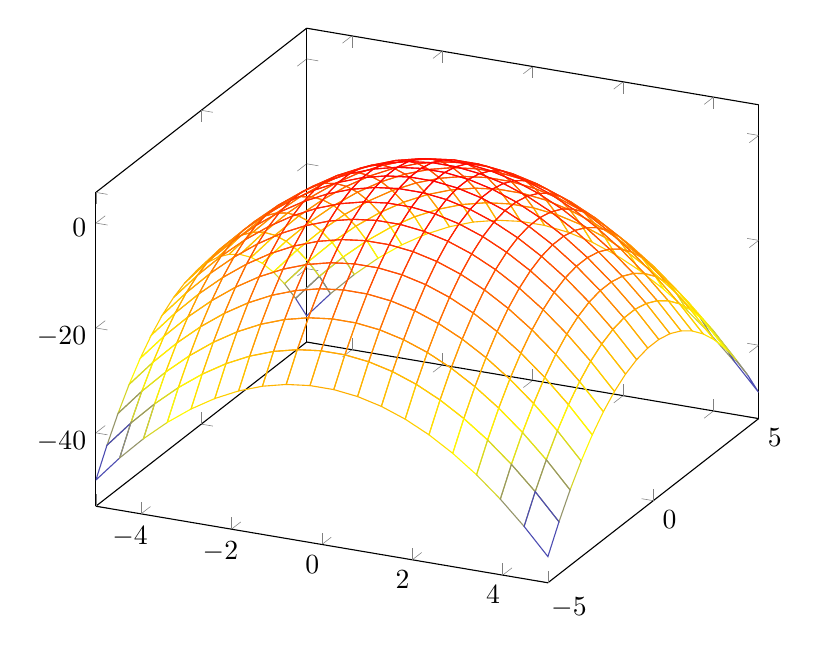
\begin{tikzpicture}
    \begin{axis}
        \addplot3[mesh, samples=20]{1-x^2-y^2};
        
    \end{axis}
\end{tikzpicture}

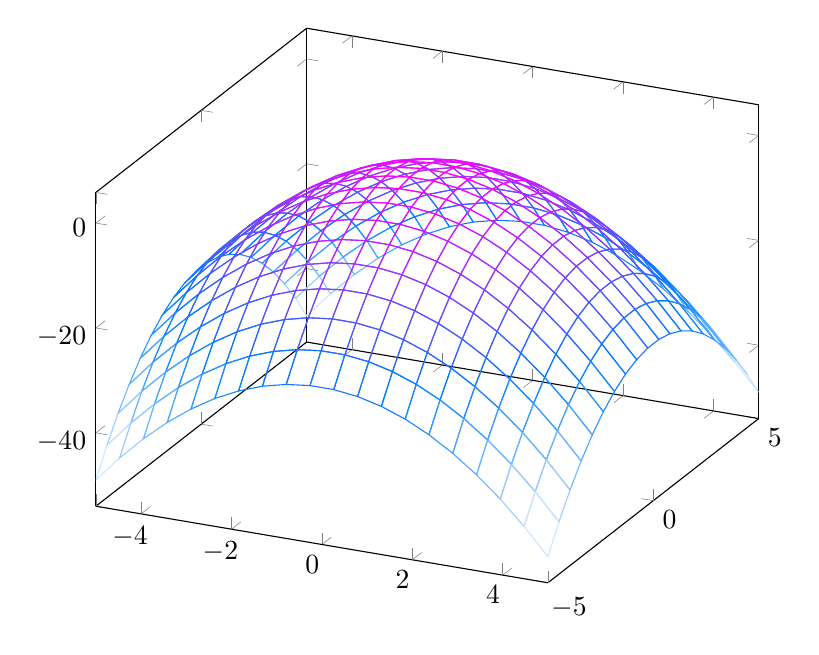
\begin{tikzpicture}
    \begin{axis}[colormap/cool]
        \addplot3[mesh, samples=20]{1-x^2-y^2};
        
    \end{axis}
\end{tikzpicture}

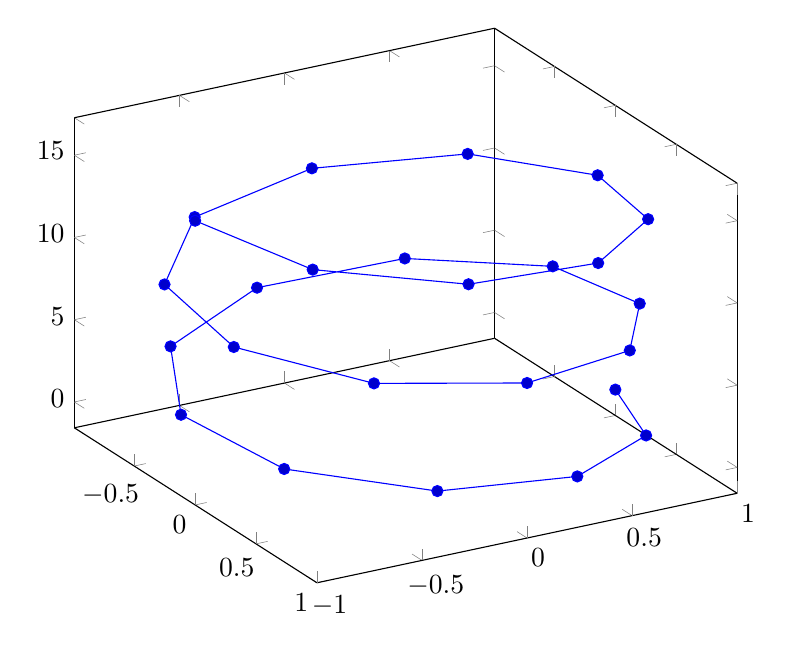
\begin{tikzpicture}
    \begin{axis}[view={60}{30}]
        \addplot3+[domain=0:5*pi, samples y=0]({sin(deg(x))}, {cos(deg(x))}, {x});
        
    \end{axis}
\end{tikzpicture}




\end{document}